%!TEX program = xelatex
\documentclass[12pt, a4paper]{article}

\usepackage[dvipsnames]{xcolor}

\usepackage{fancyhdr}
\usepackage{extramarks}
\usepackage{amsmath}
\usepackage{amsthm}
\usepackage{amsfonts}
\usepackage{tikz}
\usepackage[plain]{algorithm}
\usepackage{algpseudocode}

\usepackage{ctex}
\usepackage{indentfirst}
\usepackage{wrapfig}
\usepackage{upgreek}
\ctexset {today=old}
\usetikzlibrary{automata,positioning,shapes.geometric,arrows.meta,patterns,calc}
\numberwithin{equation}{section}

%
% Basic Document Settings
%

\topmargin=-0.25in
\evensidemargin=0in
\oddsidemargin=0in
\textwidth=6.5in
\textheight=9.2in
\headsep=0.25in

\linespread{1.1}

\pagestyle{fancy}
\lhead{\hmwkAuthorName}
\chead{\hmwkClass : \hmwkTitle}
\rhead{\firstxmark}
\lfoot{\lastxmark}
\cfoot{\thepage}

\renewcommand\headrulewidth{0.4pt}
\renewcommand\footrulewidth{0.4pt}

\setlength{\parindent}{2em}  % 2em代表首行缩进两个字符

%
% Create Problem Sections
%

\newcommand{\enterProblemHeader}[1]{
    \nobreak\extramarks{}{Problem \arabic{#1} continued on next page\ldots}\nobreak{}
    \nobreak\extramarks{Problem \arabic{#1} (continued)}{Problem \arabic{#1} continued on next page\ldots}\nobreak{}
}

\newcommand{\exitProblemHeader}[1]{
    \nobreak\extramarks{Problem \arabic{#1} (continued)}{Problem \arabic{#1} continued on next page\ldots}\nobreak{}
    \stepcounter{#1}
    \nobreak\extramarks{Problem \arabic{#1}}{}\nobreak{}
}

% \setcounter{secnumdepth}{0}
\newcounter{partCounter}
\newcounter{homeworkProblemCounter}
\setcounter{homeworkProblemCounter}{0}
% \nobreak\extramarks{Problem \arabic{homeworkProblemCounter}}{}\nobreak{}

%
% Homework Problem Environment
%
% This environment takes an optional argument. When given, it will adjust the
% problem counter. This is useful for when the problems given for your
% assignment aren't sequential. See the last 3 problems of this template for an
% example.
%
\newenvironment{homeworkProblem}[1][-1]{
    \ifnum#1>0
        \setcounter{homeworkProblemCounter}{#1}
    \fi
    \section{Problem \arabic{homeworkProblemCounter}}
    \setcounter{partCounter}{1}
    \enterProblemHeader{homeworkProblemCounter}
}{
    \exitProblemHeader{homeworkProblemCounter}
}

%
% Homework Details
%   - Title
%   - Due date
%   - Class
%   - Section/Time
%   - Instructor
%   - Author
%

\newcommand{\hmwkTitle}{Newton's laws of motion}
\newcommand{\hmwkDueDate}{\today}
\newcommand{\hmwkClass}{University Physics}
\newcommand{\hmwkClassTime}{}
\newcommand{\myUniversiy}{Wuhan University}
\newcommand{\hmwkAuthorName}{\textbf{Lai Wei}}

%
% Title Page
%

\title{
    \vspace{2in}
    \textmd{\textbf{\hmwkClass:\ \hmwkTitle}}\\
    \normalsize\vspace{0.1in}\small{Date: \hmwkDueDate}\\
    \vspace{0.1in}\large{\textit{\myUniversiy}}
    \vspace{3in}
}

\author{\hmwkAuthorName}
\date{}

\renewcommand{\part}[1]{\textbf{\large Part \Alph{partCounter}}\stepcounter{partCounter}\\}

%
% Various Helper Commands
%

% Useful for algorithms
\newcommand{\alg}[1]{\textsc{\bfseries \footnotesize #1}}

% % For derivatives
% \newcommand{\deriv}[1]{\frac{\mathrm{d}}{\mathrm{d}x} (#1)}

% For partial derivatives
\newcommand{\pderiv}[2]{\frac{\partial}{\partial #1} (#2)}

% Integral dx
\newcommand{\dx}{\mathrm{d}x}

% Alias for the Solution section header
\newcommand{\solution}{\textbf{\large Solution}}

% Probability commands: Expectation, Variance, Covariance, Bias
\newcommand{\E}{\mathrm{E}}
\newcommand{\Var}{\mathrm{Var}}
\newcommand{\Cov}{\mathrm{Cov}}
\newcommand{\Bias}{\mathrm{Bias}}

% 我的newcommand
\newcommand{\degree}{^{\circ}}
\newcommand{\arrow}{-{Stealth[length=4mm,width=2mm]}}
\newcommand{\rmd}{\mathrm{~d}}
\newcommand{\deriv}[2]{\frac{\rmd #1}{\rmd #2}}
\renewcommand{\parallel}{\mathrel{/\mskip-2.5mu/}}

\begin{document}

\maketitle

\pagebreak

% 设置页码格式是罗马数字
\pagenumbering{roman}

% 生成目录
\tableofcontents

\pagebreak

% 设置页码格式是阿拉伯数字
\pagenumbering{arabic}

\pagebreak

\section{牛顿定律}

\subsection{牛顿第一定律}

    牛顿第一定律,又称惯性定律(law of inertia) 可表述如下:任何物体都将保持静止
    或匀速直线运动的状态,直至其他物体的作用强迫它改变这种状态时为止。

    即当\(\overrightarrow{F} = 0\)时,\(\overrightarrow{v}\)为恒矢量。

    牛顿第一定律指出了两个重要概念\textbf{惯性}和\textbf{力}。

\subsection{牛顿第二定律}

\subsubsection{表述}

    动量为\(\overrightarrow{p}\)的物体, 在合外力\(\overrightarrow{F} \left(=\sum \overrightarrow{F_{i}}\right)\)
    的作用下,其动量随时间的变化率应当等于作用于物体的合外力,即

    \begin{align}
        \overrightarrow{F}\left(t\right) = \deriv{\overrightarrow{p}\left(t\right)}{t} =
        \deriv{\left(m\overrightarrow{v}\right)}{t}
    \end{align}

    (当\(v\ll c\)时,\(m\)为常量)

    于是有

    \begin{align}
        \overrightarrow{F} = m \deriv{\overrightarrow{v}}{t} = m \overrightarrow{a}
    \end{align}

    即可叙述如下:物体受到外力作用时,它所获得的加速度的大小与外力的大小成正比,
    与物体的质量成反比,加速度的方向与外力的方向相同。

\subsubsection{牛顿运动定律的矢量性}

    由

    \begin{align*}
        \overrightarrow{F} = m \deriv{\overrightarrow{v}}{t} = m \overrightarrow{a}
    \end{align*}

    得

    \begin{equation}
        \overrightarrow{F}=m \frac{\mathrm{~d} v_x}{\mathrm{~d} t} \overrightarrow{i}+m \frac{\mathrm{~d} v_y}{\mathrm{~d} t} \overrightarrow{j}+m \frac{\mathrm{~d} v_z}{\mathrm{~d} t} \overrightarrow{k}
    \end{equation}

    即

    \begin{equation}
        \overrightarrow{F}=m a_x \overrightarrow{i}+m a_y \overrightarrow{j}+m a_z \overrightarrow{k}
    \end{equation}

    所以

    \begin{equation}
        \left\{\begin{array}{l}
        F_x=m a_x \\
        F_y=m a_y \\
        F_z=m a_z
        \end{array}\right.
    \end{equation}

\subsubsection{自然坐标系中}

    \begin{equation}
        \overrightarrow{F}=m \overrightarrow{a}=
        m\left(\overrightarrow{a}_{\mathrm{t}}+\overrightarrow{a}_{\mathrm{n}}\right)=
        m \frac{\mathrm{~d} v}{\mathrm{~d} t} \overrightarrow{e}_{\mathrm{t}}+m \frac{v^2}{\rho} \overrightarrow{e}_{\mathrm{n}}
    \end{equation}

    也可写作

    \begin{equation}
        \left\{\begin{array}{l}
        F_{\mathrm{t}}=m \frac{\mathrm{~d} v}{\mathrm{~d} t}=m \frac{\mathrm{~d} s^2}{\mathrm{~d} t^2} \\
        F_{\mathrm{n}}=m \frac{v^2}{\rho}
        \end{array}\right.
    \end{equation}

    (\(\rho\)为\(A\)处曲线的曲率半径)

\subsubsection{力的叠加原理}

    当一个物体同时受到几个力的作用时,则这些力的合力产生的加逃度等于每个力单独作用时产生的矢
    量和,这一结论称为力的\textbf{独立性原理}或\textbf{力的叠加原理}。

    即

    \begin{equation}
        \begin{aligned}
        \overrightarrow{F} & =\overrightarrow{F}_1+\overrightarrow{F}_2+\cdots+\overrightarrow{F}_n=\sum \overrightarrow{F}_i \\
        & =m \overrightarrow{a}_1+m \overrightarrow{a}_2+\cdots+m \overrightarrow{a}_n=m \sum \overrightarrow{a}_i=m \overrightarrow{a}=m \frac{\mathrm{~d} v}{\mathrm{~d} t}
        \end{aligned}
    \end{equation}

\subsection{牛顿第三定律}

    两个物体之间作用力\(\overrightarrow{F}\)反和反作用力\(\overrightarrow{F}^{'}\), 
    沿同一直线,大小相等,方向相反,分别作用在两个物体上。

    作用力和反作用力的特点:

    \begin{enumerate}
        \item 作用力与反作用力总是同时存在、相互依存的。
        \item 作用力与反作用力分别作用在两个不同的物体上,虽然它们大小相等、方向相反,但不能互相抵消。
        \item 作用力与反作用力一定属于同一性质的力。
    \end{enumerate}

\subsection{总结}

    \begin{enumerate}
        \item 凡相对于惯性系作匀速直线运动的一切参考系都是惯性系;
        \item 对于不同惯性系,牛顿力学的规律都具有相同的形式,与惯性系的运动无关。
            (\textbf{伽利略相对性原理}或称\textbf{力学相对性原理})
    \end{enumerate}

\section{非惯性系、惯性力}

\subsection{惯性系、非惯性系}

\subsubsection{惯性系}

    牛顿运动定律在其中成立的参考系称为\textbf{惯性参考系},简称\textbf{惯性系}(inertial system)。

    “一个远离其他一切物体,而且没有自转的物体是惯性参照系,一切相对于该物体做匀速直线运动的参照系也是惯性参照系。
    牛顿定律就是在这样的参照系中成立。”——王燕生教授《大学物理问题讨论集》

    \textbf{举例}:

    \begin{enumerate}
        \item 地面参考系;
        \item 地心参考系;
        \item 日心参考系;
        \item FK4参考系:以选定的1535颗恒星的平均静止的位形作为基准的参考系,是比以上三个参考系都严格的惯性系。
    \end{enumerate}

\subsubsection{非惯性系}

    牛顿运动定律不成立的参考系称为\textbf{非惯性系}(non-inertial system)。

\subsection{惯性力}

\subsection{平动加速参考系、平动惯性力}

\subsubsection{定义}

    假设非惯性系K'相对于惯性系K以加速度\(\overrightarrow{a}_{0}\)做平动,则由相对运动规律可知,质点相对于
    K'系和K系的加速度\(\overrightarrow{a}_{0}\)和\(\overrightarrow{a}\)满足:

    \begin{align}
        \overrightarrow{a} = \overrightarrow{a}_{0} + \overrightarrow{a}^{'}
    \end{align}

    惯性系中K,牛顿运动定律成立,即

    \begin{align}
        \overrightarrow{F} = m \overrightarrow{a} = m \left(\overrightarrow{a}_{0} + \overrightarrow{a}^{'}\right)
    \end{align}

    移项,得

    \begin{align}
        \overrightarrow{F} - m\overrightarrow{a}^{'} =  m \overrightarrow{a}_{0}
    \end{align}

    定义\textbf{平动惯性力}:

    \begin{align}
        \overrightarrow{F}_{0} = - m\overrightarrow{a}^{0}
    \end{align}

    将\(\overrightarrow{F}^{'} = \overrightarrow{F} + \overrightarrow{F}_{0} = \overrightarrow{F} -
    m \overrightarrow{a}_{0}\)看作非惯性参考系中受到的“合外力”,则在非惯性系K'中,牛顿第二定律在形式上成立:

    \begin{align}
        \overrightarrow{F}^{'} = \overrightarrow{F} + \overrightarrow{F}_{0} = m \overrightarrow{a}^{'}
    \end{align}

\subsubsection{性质}

    不是真实的力,无施力物体,无反作用力是非惯性系加速度的反映。

\subsection{匀速转动参考系、惯性离心力}
    
    \begin{wrapfigure}{r}{4cm}
        \centering
        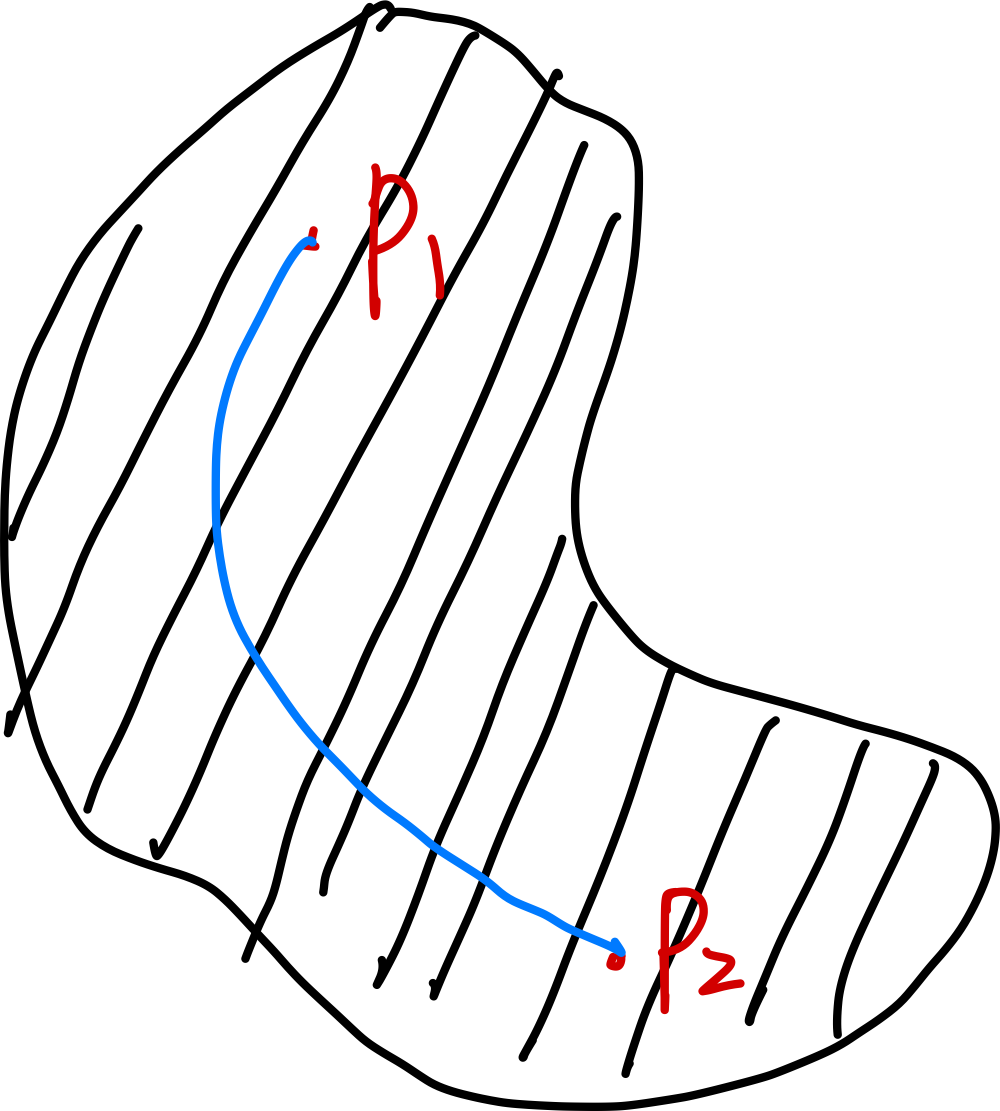
\includegraphics[scale=0.2]{"Chapter 02 images/pic1.jpg"}
        % \caption{}
        \label{pic1}
    \end{wrapfigure}

    匀速转动参考系也是一种常见的非惯性系。如右图所示,水平转盘以匀角速度\(\omega\)绕通过圆心的垂直轴转动,
    质量为\(m\)的小球用长度为\(R\)的绳子与转轴相连静止在圆盘上,并随圆盘一起转动。站在地面上的观察者看来,
    小球\(m\)以匀角速度\(\omega\)随圆盘一起转动,绳子施于小球的拉力\(\overrightarrow{F}_{r}\)
    提供了小球做匀速圆周运动时所需的向心力,即

    \begin{align}
        \overrightarrow{F}_{\mathrm{T}}=-m \frac{v^2}{R} \overrightarrow{e}_r=-m \omega^2 R \overrightarrow{e}_r
    \end{align}

    这表明在地面参考系中,小球的运动符合牛顿运动定律。

    但是,从圆盘这个转动参考系中来看,小球受到合外力\(\overrightarrow{F}_{T}\)的作用,但是静止不动。
    为了在转动参考系中,仍然能够用牛顿运动定律解释该现象,需要引入一个虛拟的惯性力\(\overrightarrow{F}_{0}\),
    该力与绳子的拉力\(\overrightarrow{F}_{T}\)大小相等、方向相反,即

    \begin{equation}
        \overrightarrow{F}_0=-\overrightarrow{F}_{\mathrm{T}}=m \omega^2 R \overrightarrow{e}_r=-m \overrightarrow{a}_{\mathrm{n}}
    \end{equation}

    (\(\overrightarrow{e}_r\)表示径向单位矢量)

    称为\textbf{惯性离心力}(inertial centrifugal force)。

    于是引入惯性离心力后,在转动参考系中,牛顿运动定律在形式上成立。物体受到“合外力”为

    \begin{align*}
        \overrightarrow{F}_{T} + \overrightarrow{F}_{0} = \overrightarrow{0}
    \end{align*}

\section{例题}

\subsection{解题思路}

    牛顿定律主要处理两类问题:

    \begin{enumerate}
        \item 质点;
        \item 质点系,尤其是连续分布的质点系。
    \end{enumerate}

    解题的基本思路:

    \begin{enumerate}
        \item 确定研究对象进行受力分析(隔离物体,画受力图);
        \item 取坐标系;
        \item 列方程(一般用分量式);
        \item 利用其它的约束条件列补充方程;
        \item 先用文字符号求解,后带入数据计算结果。
    \end{enumerate}

\subsection{Problem 1}

    一质量\(m\),半径\(r\)的球体在水中静止释放沉入水底。已知阻力\(F_{r} = - 6 \uppi r \eta v\),
    \(\eta\)为粘滞系数,求\(v\left(t\right)\)。
    \vspace{1em}

    \textbf{Solution}
    \vspace{1em}

    \begin{wrapfigure}{r}{4cm}
        \centering
        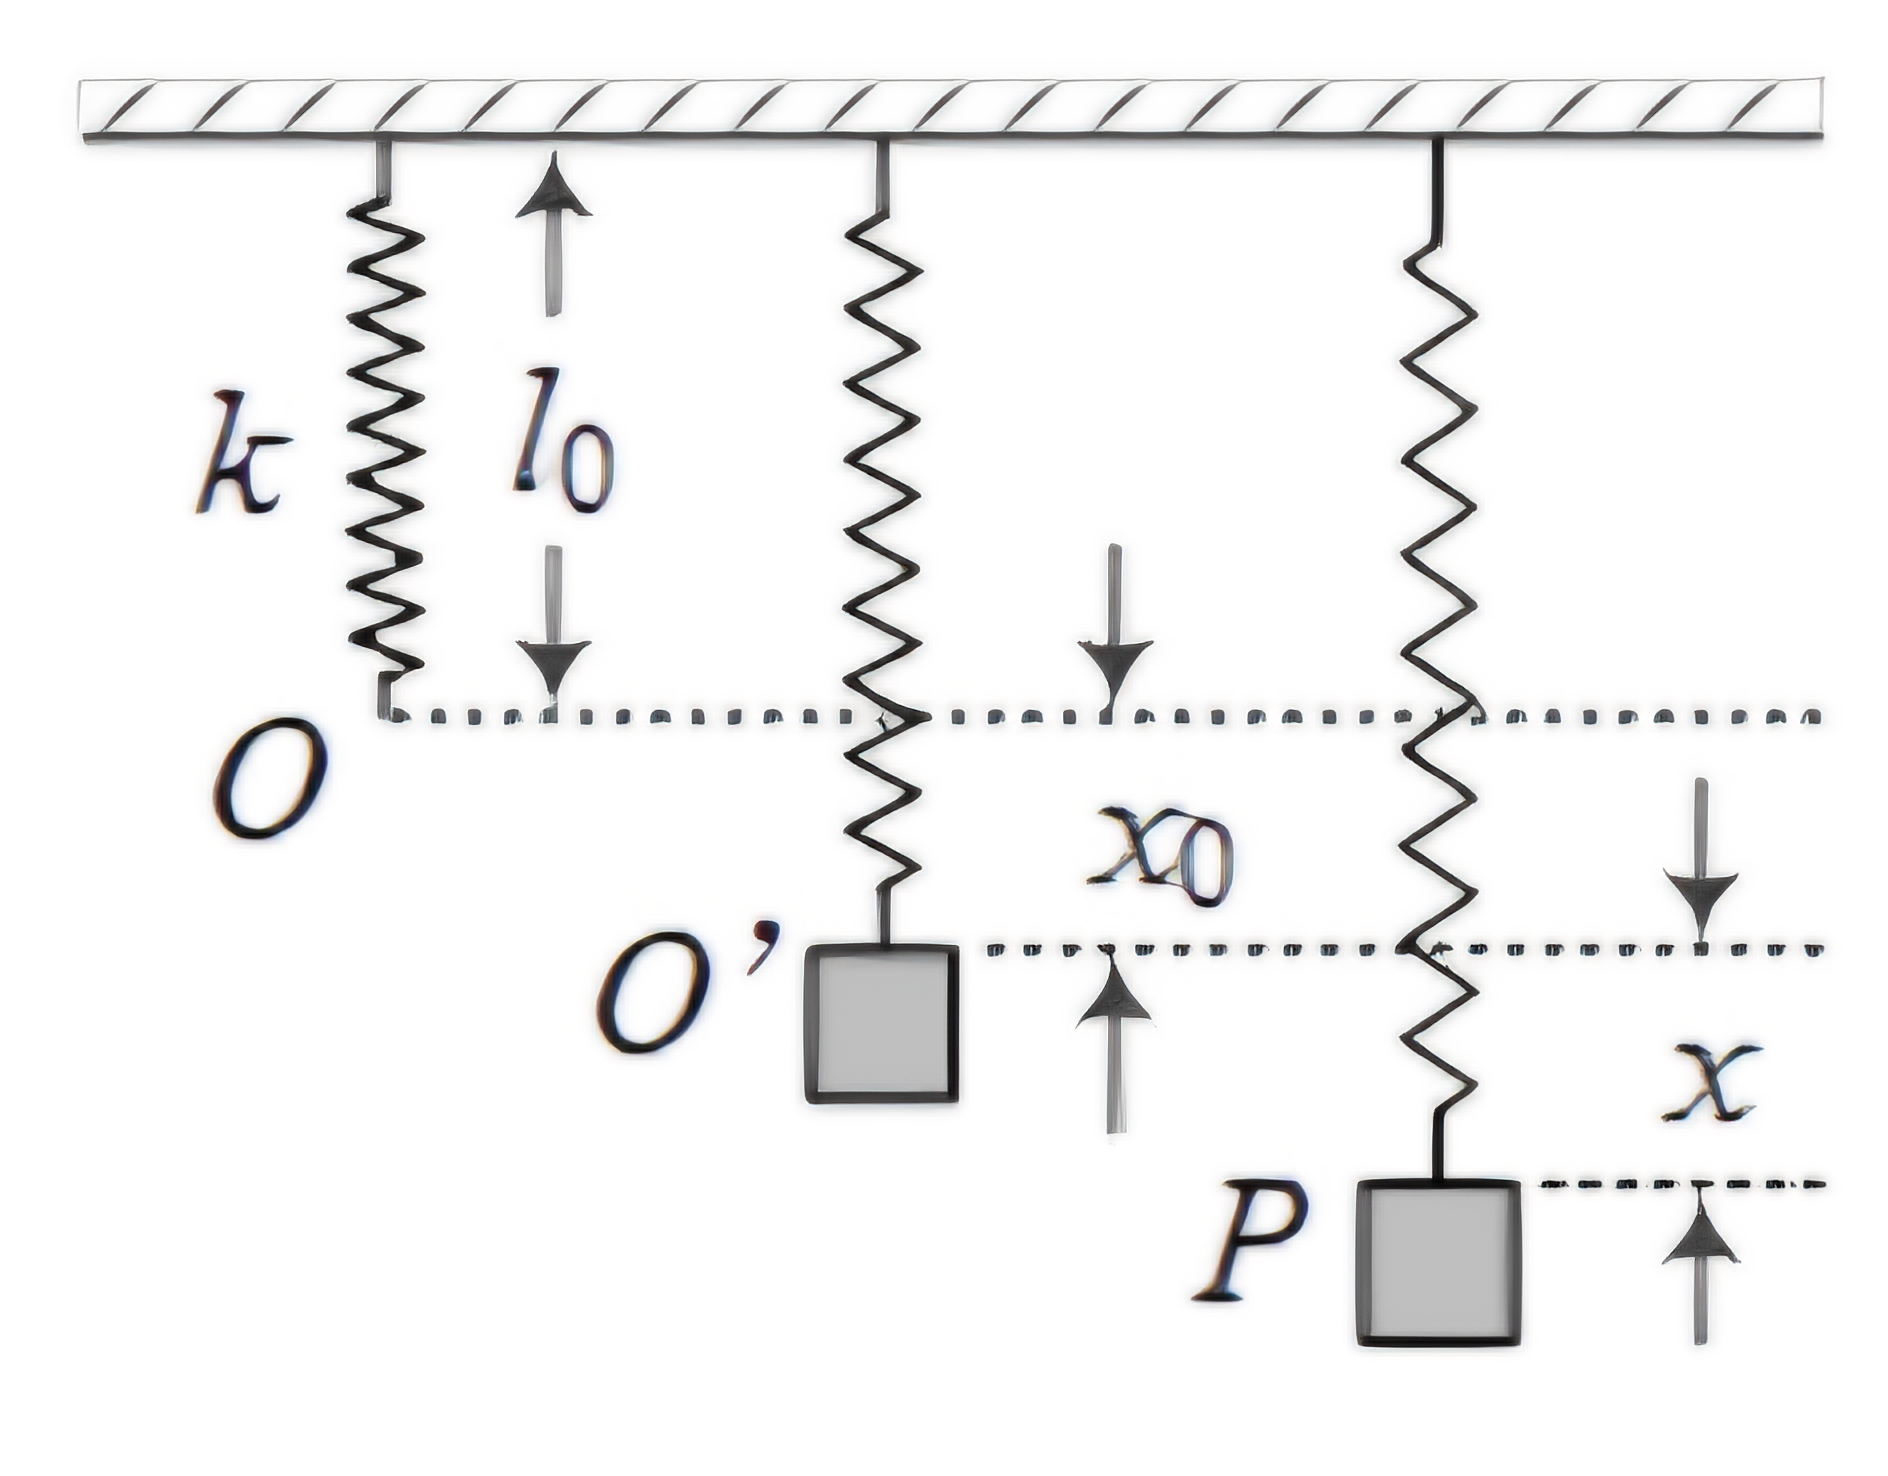
\includegraphics[scale=0.3]{"Chapter 02 images/pic2.png"}
        % \caption{}
        \label{pic2}
    \end{wrapfigure}

    取坐标如图(\(\overrightarrow{F}_{B}\)为浮力),则

    $$
        m g-F_{\mathrm{B}}-6 \uppi \eta r v=m a
    $$

    令\(F_{0} = mg - F_{B}\),\(b = 6 \uppi \eta r\),于是

    $$
        F_0-b v=m \frac{\mathrm{~d} v}{\mathrm{~d} t}
    $$

    即

    $$
        \frac{\mathrm{d} v}{\mathrm{~d} t}=-\frac{b}{m}\left(v-\frac{F_0}{b}\right)
    $$

    两边同时积分:

    $$
        \int_0^v \frac{\rmd v}{v-\left(\frac{F_0}{b}\right)}=-\frac{b}{m} \int_0^t \rmd t
    $$

    得

    $$
        v=\frac{F_0}{b}\left[1-\mathrm{e}^{-\frac{b}{m} t}\right]
    $$

    \begin{wrapfigure}{r}{4cm}
        \centering
        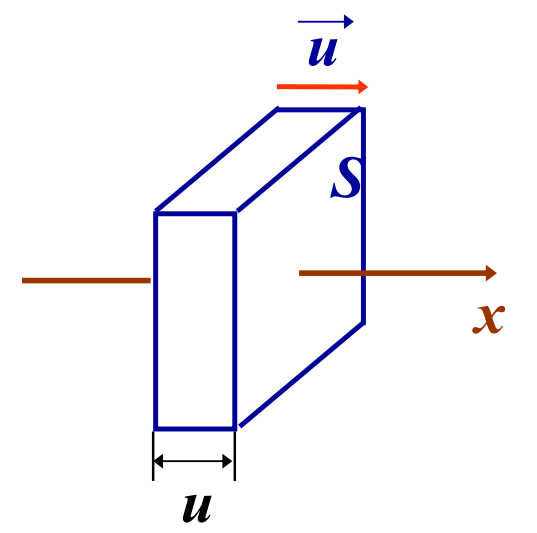
\includegraphics[scale=0.3]{"Chapter 02 images/pic3.png"}
        % \caption{}
        \label{pic3}
    \end{wrapfigure}

    则当\(t \rightarrow \infty\)时,\(v_{L} \rightarrow \frac{F_{0}}{b}\)(极限速度),
    当\(t = 3 \frac{b}{m}\)时,\(v = v_{L}\left(1-0.05\right) = 0.95 v_{L}\)。
    一般认为\(t \leq 3 \frac{b}{m}\)时,\(v = v_{L}\)

\subsection{Problem 2}

    质量为\(m\)的物体,由地面以初速度\(v_{0}\)竖直向上发射,物体受到空气阻力大小\(F_{r} = kv\)。
    试求:

    \begin{enumerate}
        \item 物体发射到最大高度所需要的时间;
        \item 物体能到达的最大高度。
    \end{enumerate}

    \textbf{Solution}
    \\

    \textbf{Part One}
    \\

    \begin{wrapfigure}{r}{4cm}
        \centering
        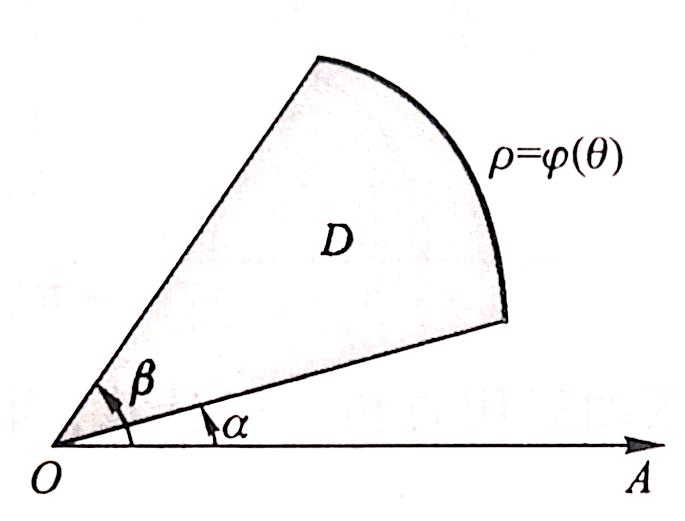
\includegraphics[scale=0.3]{"Chapter 02 images/pic4.png"}
        % \caption{}
        \label{pic4}
    \end{wrapfigure}

    物体在向上发射的过程中,受到重力和阻力作用,方向均与速度方向相反。以竖直向上作为正方向,
    由牛顿运动定律可得

    \begin{equation}
        -m g-k v=m \frac{\mathrm{~d} v}{\mathrm{~d} t}
        \label{Problem-2-1}
    \end{equation}

    对上式分离变量并取定积分,同时注意到物体到达最大高度时\(v=0\),即

    $$
        \int_0^t \mathrm{~d} t=\int_{v_0}^0-\frac{m}{m g+k v} \mathrm{~d} v
    $$

    积分得物体达到最大高度所需的时间为

    $$
        t=\frac{m}{k} \ln \frac{m g+k v_0}{m g}
    $$

    \textbf{Part Two}
    \\

    利用$\dfrac{\mathrm{d} v}{\mathrm{~d} t}=v \dfrac{\mathrm{~d} v}{\mathrm{~d} y}$代入\ref{Problem-2-1}式,可得

    $$
        -m g-k v=m \frac{\mathrm{~d} v}{\mathrm{~d} t}
    $$

    分离变量并取定积分,即

    $$
        \int_0^y \mathrm{~d} y=\int_{v_0}^0-\frac{m v}{m g+k v} \mathrm{~d} v
    $$

    所以物体可达到的最大高度为

    $$
        y=\frac{m}{k}\left(v_0-\frac{m g}{k} \ln \frac{m g+k v_0}{m g}\right)
    $$

\subsection{Problem 3}

    \begin{wrapfigure}{r}{4cm}
        \centering
        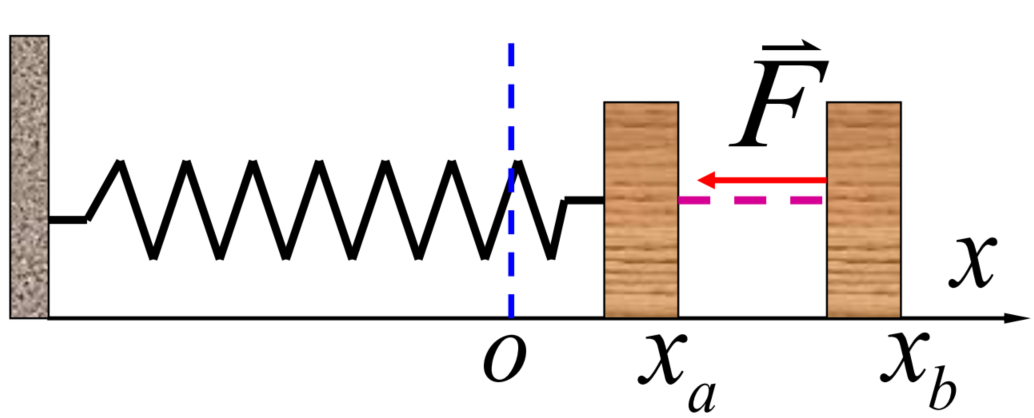
\includegraphics[scale=0.18]{"Chapter 02 images/pic5.png"}
        % \caption{}
        \label{pic5}
    \end{wrapfigure}

    一条质量均匀分布的绳子,总质量为\(M\)、长度为\(L\),一端拴在竖直转轴\(OO^{'}\)上,
    并以恒定的角速度\(\omega\)在水平面上旋转。设转动过程中绳子始终伸直不打弯,
    且忽略重力的影响,求距离转轴为\(r\)处绳中的张力\(T\left(r\right)\)。
    \\

    \textbf{Solution}
    \\

    在距离转轴为\(r\)处,取一个长为\(\rmd r\)的一小段绳子,其质量为\(\frac{M}{L} \rmd r\),
    其两端受力如图所示,由于该段绳子作圆周运动,所以由牛顿第二定律得

    \begin{wrapfigure}{r}{4cm}
        \centering
        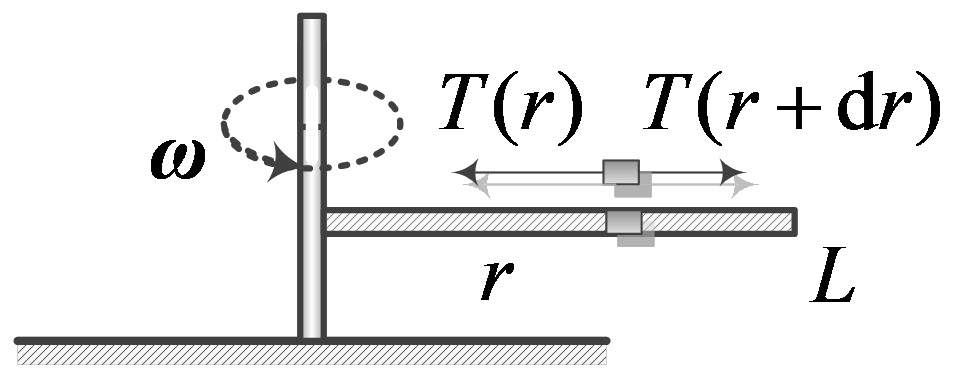
\includegraphics[scale=0.18]{"Chapter 02 images/pic6.png"}
        % \caption{}
        \label{pic6}
    \end{wrapfigure}

    $$
        T(r)-T(r+\rmd r)=\rmd m \cdot a_n=\frac{M}{L} \rmd r
    $$

    令

    $$
        T(r)-T(r+\rmd r)=\rmd m \cdot a_n=\frac{M}{L} \rmd r
    $$

    得

    $$
        \rmd T=-\frac{M \omega^2}{L} r \rmd r
    $$

    式中\(\rmd T\)就是该小段绳子所受的合外力,“\(-\)”号表示该段绳子受到的合外力的方向与矢径
    \(r\)相反,指向圆心。根据力的叠加原理,离轴\(r\)处绳中的张力就是\(r\)以外所有小段绳子所受的
    合力的绝对值之和,即

    $$
        T(r)=\int|\mathrm{d} T|=\int_r^L \frac{M \omega^2}{L} r \mathrm{~d} r=\frac{M \omega^2}{2 L}\left(L^2-r^2\right)
    $$

\end{document}
